\documentclass[useAMS,referee]{biom}

\graphicspath{{~/temp/rna-seq-stan/fig-rm-stan_laplace}}
%%%%% PLACE YOUR OWN MACROS HERE %%%%%

\def\bSig\mathbf{\Sigma}
\newcommand{\VS}{V\&S}
\newcommand{\tr}{\mbox{tr}}

\title[Empirical Bayes analysis for detection of gene heterosis in RNAseq data]{Empirical Bayes analysis for detection of gene heterosis in RNAseq data}

\author{Jarad Niemi $^*$\email{niemi@iastate.edu}, 
Eric Mittman, 
Will Landau, and 
Dan Nettleton \\
Department of Statistics, Iowa State University, Ames, Iowa, U.S.A.}

\begin{document}

\date{{\it Received December} 2014} 

\pagerange{\pageref{firstpage}--\pageref{lastpage}} 
\volume{VV}
\pubyear{YYYY}
\artmonth{Month}
\doi{}

\label{firstpage}

%  put the summary for your paper here

\begin{abstract}
This is the summary for this paper.
\end{abstract}

\begin{keywords}
Empirical Bayes; Heterosis; Hierarchical Model; Negative binomial; RNAseq.
\end{keywords}

\maketitle

%  A maximum of six (6) tables or figures combined is often required.''

\section{Introduction}
\label{s:intro}

\section{Heterosis}
\label{s:heterosis}

\section{Hierarchical model for RNAseq}
\label{s:model}


\section{Empirical Bayes}
\label{s:inf}

\section{Simulation study}
\label{s:simulation}

\subsection{Coverage for our model}



\subsection{Heterosis detection}

\begin{figure}[htbp]
\includegraphics{exampleROC0_1}
\caption{Example ROC curves for the first simulation}
\label{f:roc}
\end{figure}

\begin{figure}[htbp]
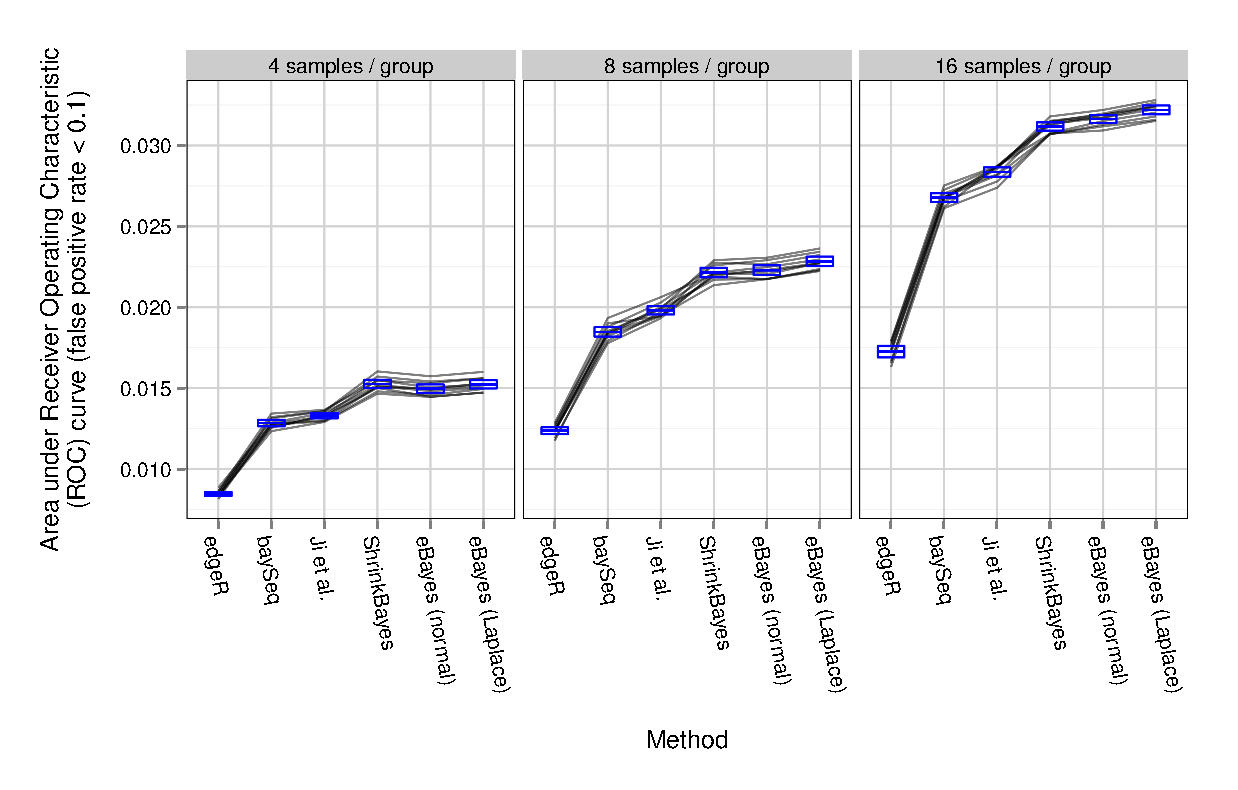
\includegraphics{auc-facet-TRUE}
\caption{Area under the ROC curves for 3 different sample sizes (facets) for the methods under comparison.}
\end{figure}

\section{Heterosis in corn ??}
\label{s:corn}

\section{Discussion}
\label{s:discuss}

Put your final comments here. 



\backmatter %  Please keep this command in your document in this position 



\section*{Acknowledgements}

The authors thank Andrew Lithio for help implementing our model in {\tt ShrinkBayes}.

%  If your paper refers to supplementary web material, then you MUST
%  include this section!!  See Instructions for Authors at the journal
%  website http://www.biometrics.tibs.org

\section*{Supplementary Materials}

Web Appendix A, referenced in Section~\ref{s:model}, is available with
this paper at the Biometrics website on Wiley Online
Library.\vspace*{-8pt}

\bibliography{jarad}
\bibliographystyle{biom}

\appendix

%  To get the journal style of heading for an appendix, mimic the following.

\section{}
\subsection{Stan model for heterosis}



\label{lastpage}

\end{document}
